\textbf{Входные параметры:}
 
Parent1 --- первый родитель;
 
Parent2 --- второй родитель;
 
VHML\_ResultVector --- потомок;
 
VHML\_N --- размер векторов Parent1, Parent2 и VHML\_ResultVector.

\textbf{Возвращаемое значение:}

 Отсутствует.
 
\textbf{ Примечание:}

 Потомок выбирается случайно.
 
 \textbf{Формула:}
\begin{align}
&Crossover \left( \overline{Parent}^1, \overline{Parent}^2, DataOfCros\right)=Random \left(\left\lbrace \overline{Offspring}^1; \overline{Offspring}^2\right\rbrace  \right), \nonumber\\
&R=Random\left( \left\lbrace 2; 3; \ldots; n\right\rbrace \right); \nonumber \\
& \overline{Offspring}^1_i=\overline{Parent}^1_i, i=\overline{1,R-1};\nonumber\\
&  \overline{Offspring}^1_i=\overline{Parent}^2_i, i=\overline{R,n};\nonumber\\
&\overline{Offspring}^2_i=\overline{Parent}^2_i, i=\overline{1,R-1};\nonumber\\
& \overline{Offspring}^2_i=\overline{Parent}^1_i, i=\overline{R,n};\nonumber\\
&\overline{Offspring}^1\in X, \overline{Offspring}^2\in X.\nonumber
\end{align}

$ DataOfCros $ не содержит каких-либо параметров относительно данного типа скрещивания.

\textbf{Пример.} Для всех видов скрещивания будем использовать двух родителей: $\overline{Parent}^1\hmm={\left( 0; 1; 0; 1; 1; 1; 0; 0\right)}^\mathrm{T}  $ и $\overline{Parent}^2={\left( 1; 1; 0; 0; 1; 0; 1\right)}^\mathrm{T}  $. Одноточечное скрещивание показано на рисунке:

\begin{figure} [h] 
  \center
  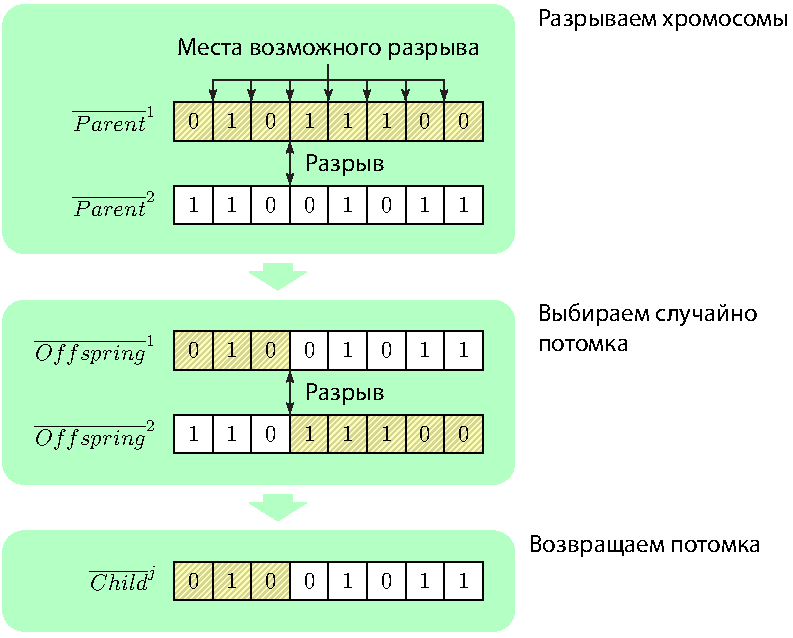
\includegraphics [scale=0.8] {HML_SinglepointCrossover_Sheme}
  \caption{Механизм работы одноточечного скрещивания} 
  \label{img:HML_SinglepointCrossover_Sheme}  
\end{figure}